\chapter{Experiment}

The experiment was conducted on the ROS bag taken during the first rehearsal attempt. The robot drove around the perimeter to map the whole arena using the Gmapping package. The brick pattern is placed in the left bottom quadrant and the drone delivery in the right top quadrant of the arena. It was surprising that the organizers chose the arena with a significant slope in the middle. We did not expect perfectly flat ground, but the angle of the slope was much higher than our expectations. Besides, the middle part of the arena was made of different - very smooth surface, which negatively influenced odometry, especially in rotation. That makes the localization in the middle much more difficult because, in this place, the robot is tilted, so the laserscan aims into the ground or into the height, and there is also a quite high distance to the nearest significant feature inside the map, which could help to adjust the position. This behavior is visible on the particle cloud during the experiment. When the robot arrives in the middle, the particles are spread into the width. These circumstances caused many problems to teams, which trained for the contest in laboratory grade conditions. Also, it is necessary to mention that there were many people inside the arena during our experiment, which makes the detection even more challenging because people could be easily interpreted as a red pile.



\begin{figure}[H]
	\centering
	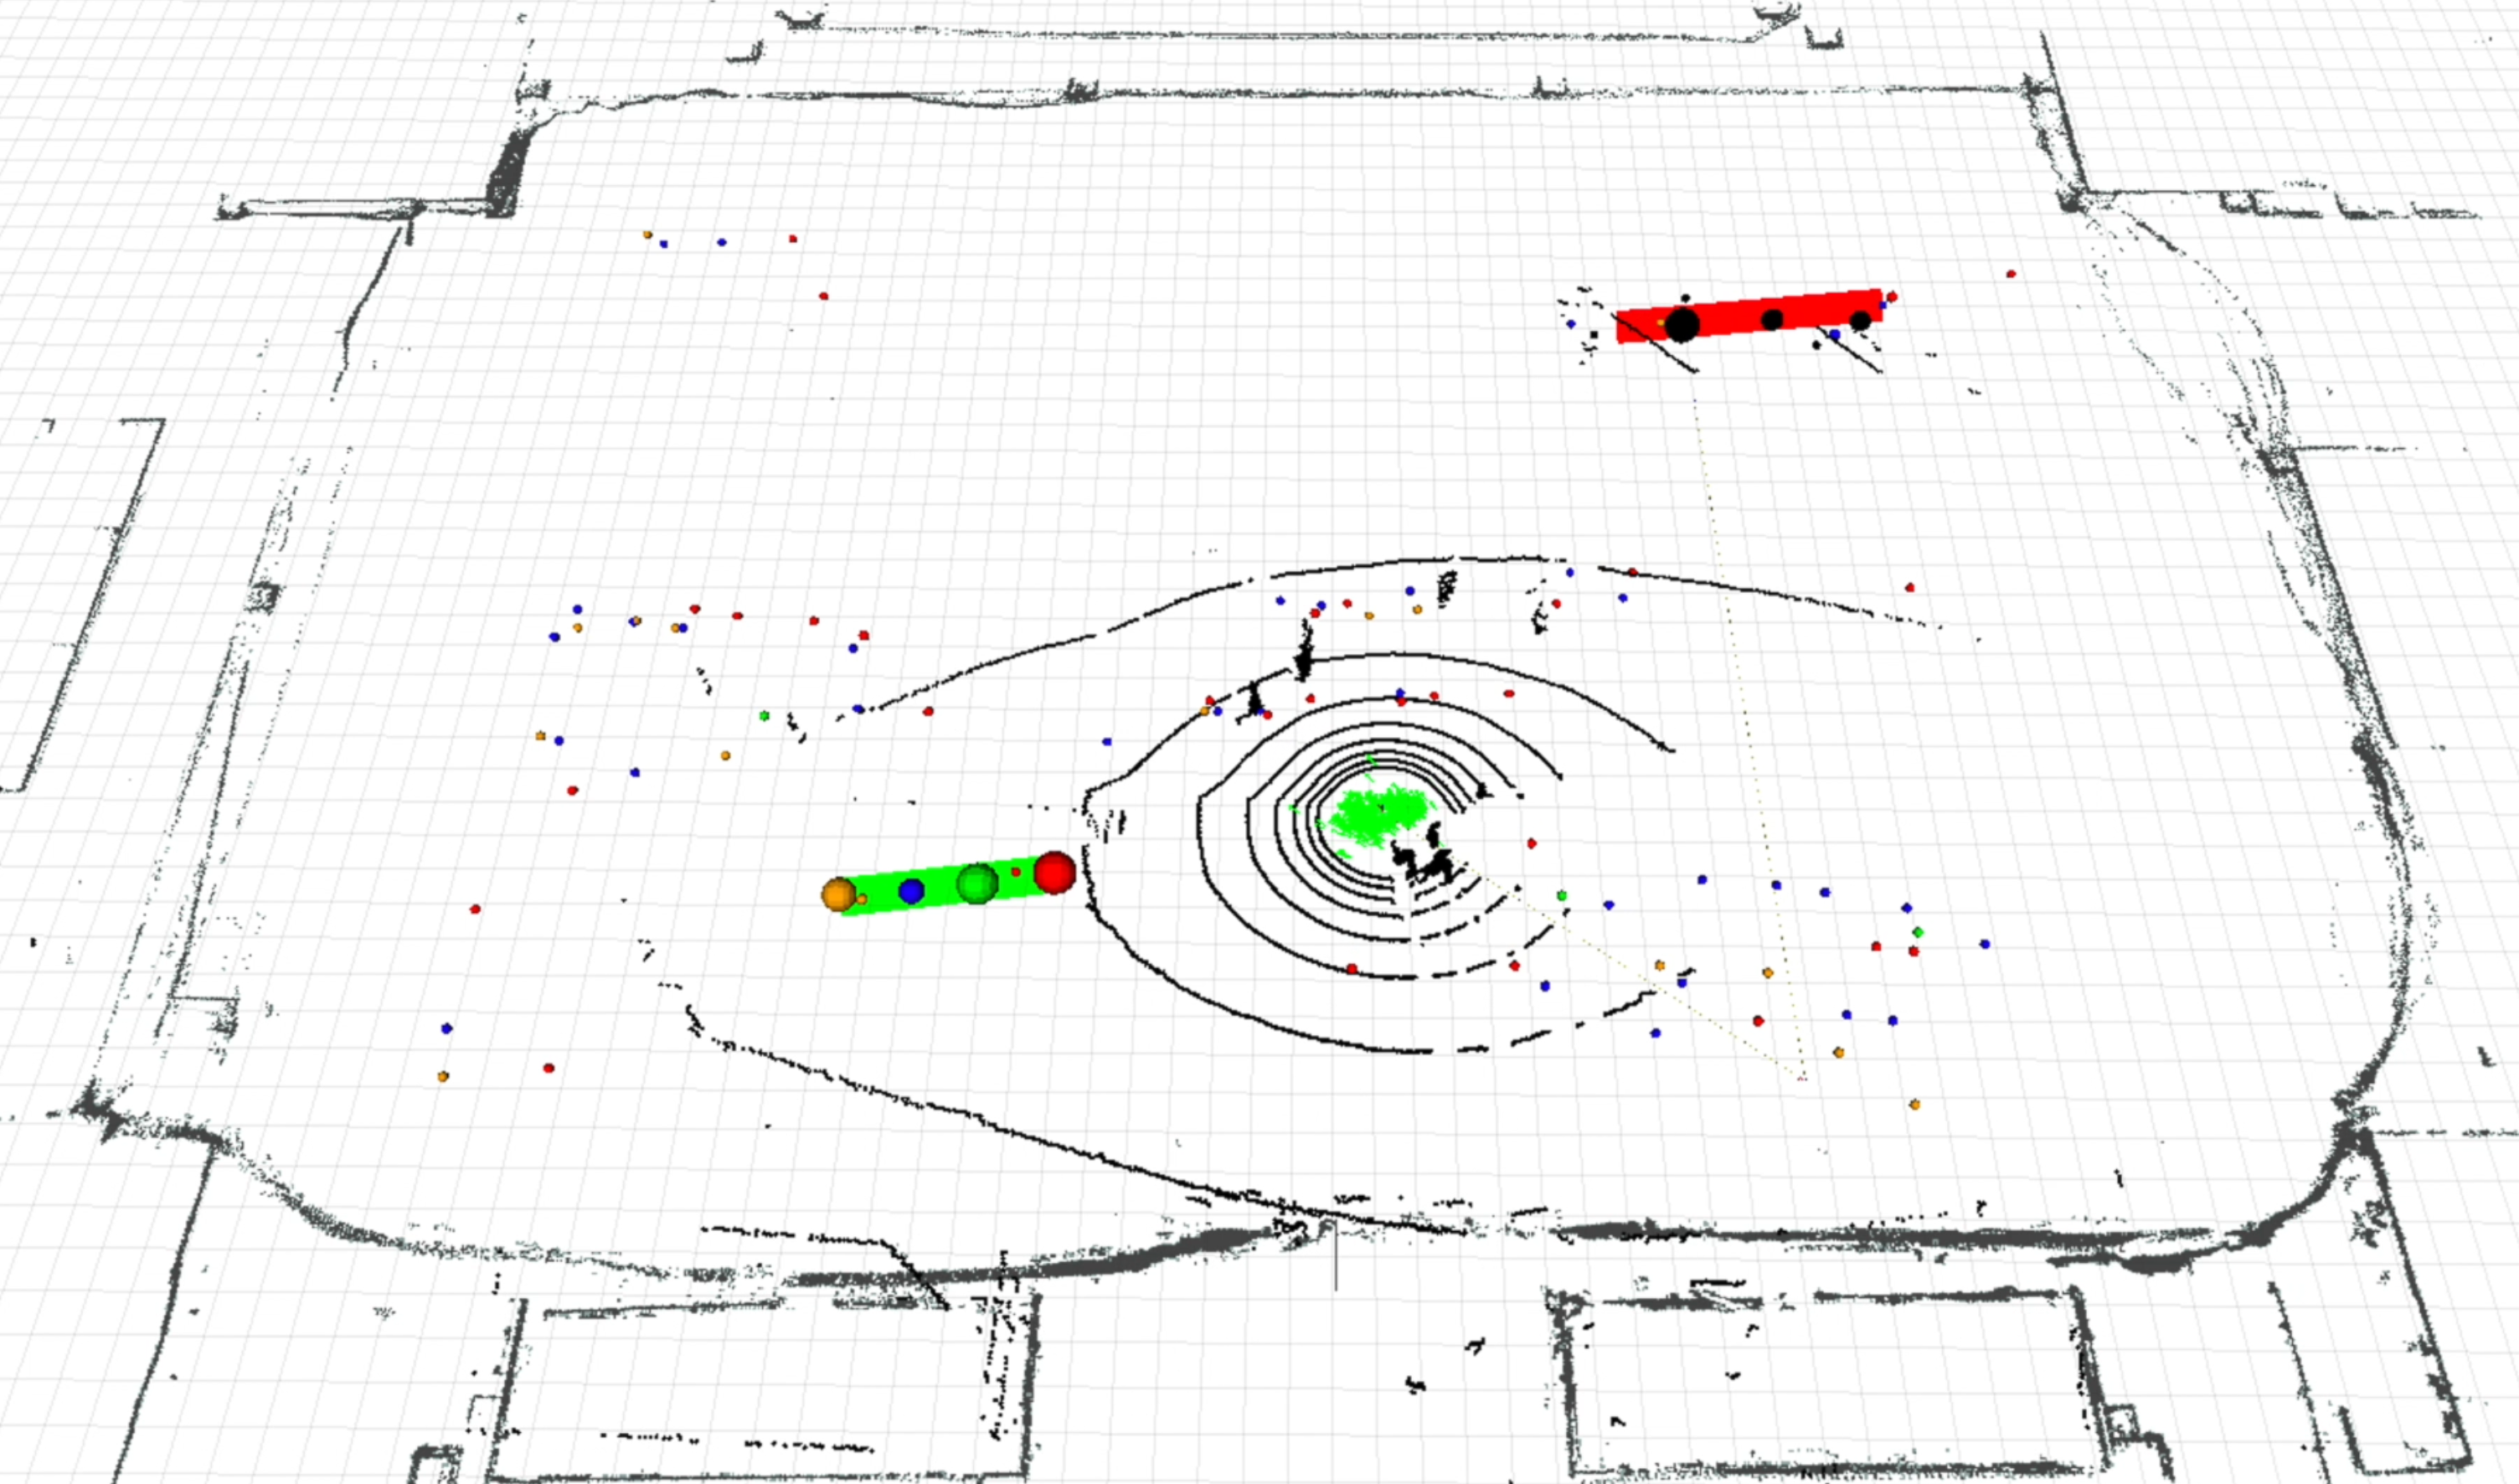
\includegraphics[scale=0.33]{fig/experiment}
	\caption[Experiment results]{In the figure is a screenshot from the experiment. Small spheres on the map are polled clusters from the symbolic map. Different types of detections create these clusters. The size of the sphere represents the confidence of a cluster. The spheres' color corresponds to the color of bricks, and the spheres representing the clusters for UAV destination are colored black. Black is also the pointcloud obtained from lidar and borders of the map. In green color are visualized all particles from the AMCL and also the line representing detection of initial brick pattern. A red line marks the position and rotation of the UAV destination. Note that the RANSAC detector was disabled in this experiment to test the EM algorithm fitting properly. The whole video from the experiment is available at \footnotemark.}
	\label{fig:experiment}
\end{figure}
\footnotetext{\url{https://www.youtube.com/watch?v=7ebl4dwkl4w} } 


\newpage